% multiple1902 <multiple1902@gmail.com>
% design.tex
% Copyright 2011~2012, multiple1902 (Weisi Dai)
% https://code.google.com/p/xjtuthesis/
% 
% It is strongly recommended that you read documentations located at
%   http://code.google.com/p/xjtuthesis/wiki/Landing?tm=6
% in advance of your compilation if you have not read them before.
%
% This work may be distributed and/or modified under the
% conditions of the LaTeX Project Public License, either version 1.3
% of this license or (at your option) any later version.
% The latest version of this license is in
%   http://www.latex-project.org/lppl.txt
% and version 1.3 or later is part of all distributions of LaTeX
% version 2005/12/01 or later.
%
% This work has the LPPL maintenance status `maintained'.
% 
% The Current Maintainer of this work is Weisi Dai.
%

\chapter{系统设计}
\echapter{Design}
\label{DesignChapter}
本系统的设计包含两个主要部分。客户端函数库的设计和应用层同步、发现、更新模块的设计。由于同步模块的功能是获取对象的名称,本文中有时也将其称为发现模块。由图\ref{fig:AbstractStructure}所示,客户端函数库为发现模块提供和操作系统、以及NDN底层组件交互的接口;而发现模块为游戏提供发现节点,更新位置的功能。

\section{客户端函数库}
\par
NDN客户端是NDN项目的重要组成部分。其为开发者提供一套和NDN的底层组件交互的接口。例如,客户端函数库对上层应用开发者应当提供“注册数据请求名称前缀(Register Prefix)”函数。函数的具体实现,如何调用语言和操作系统提供的传输层网络接口,以及和NFD的交互过程应当在客户端函数库中实现。
\par
目前的NDN客户端函数库的实现有Java,Python和C++三种语言。由于Unity3D引擎的语言选择是基于Mono Framework的,作者的工作还包括客户端函数库的C\#语言实现。
\par
设计上所有NDN客户端函数库应当提供统一的接口,遵循统一的规定。具体规范在项目的在线文档有所描述(ref)。目前的Java语言NDN客户端函数库的类图结构如图\ref{fig:CCLClassDiagram}。作者开发的C\#客户端函数库遵循同样的类图结构。
\begin{figure}[h!]
	\centering
	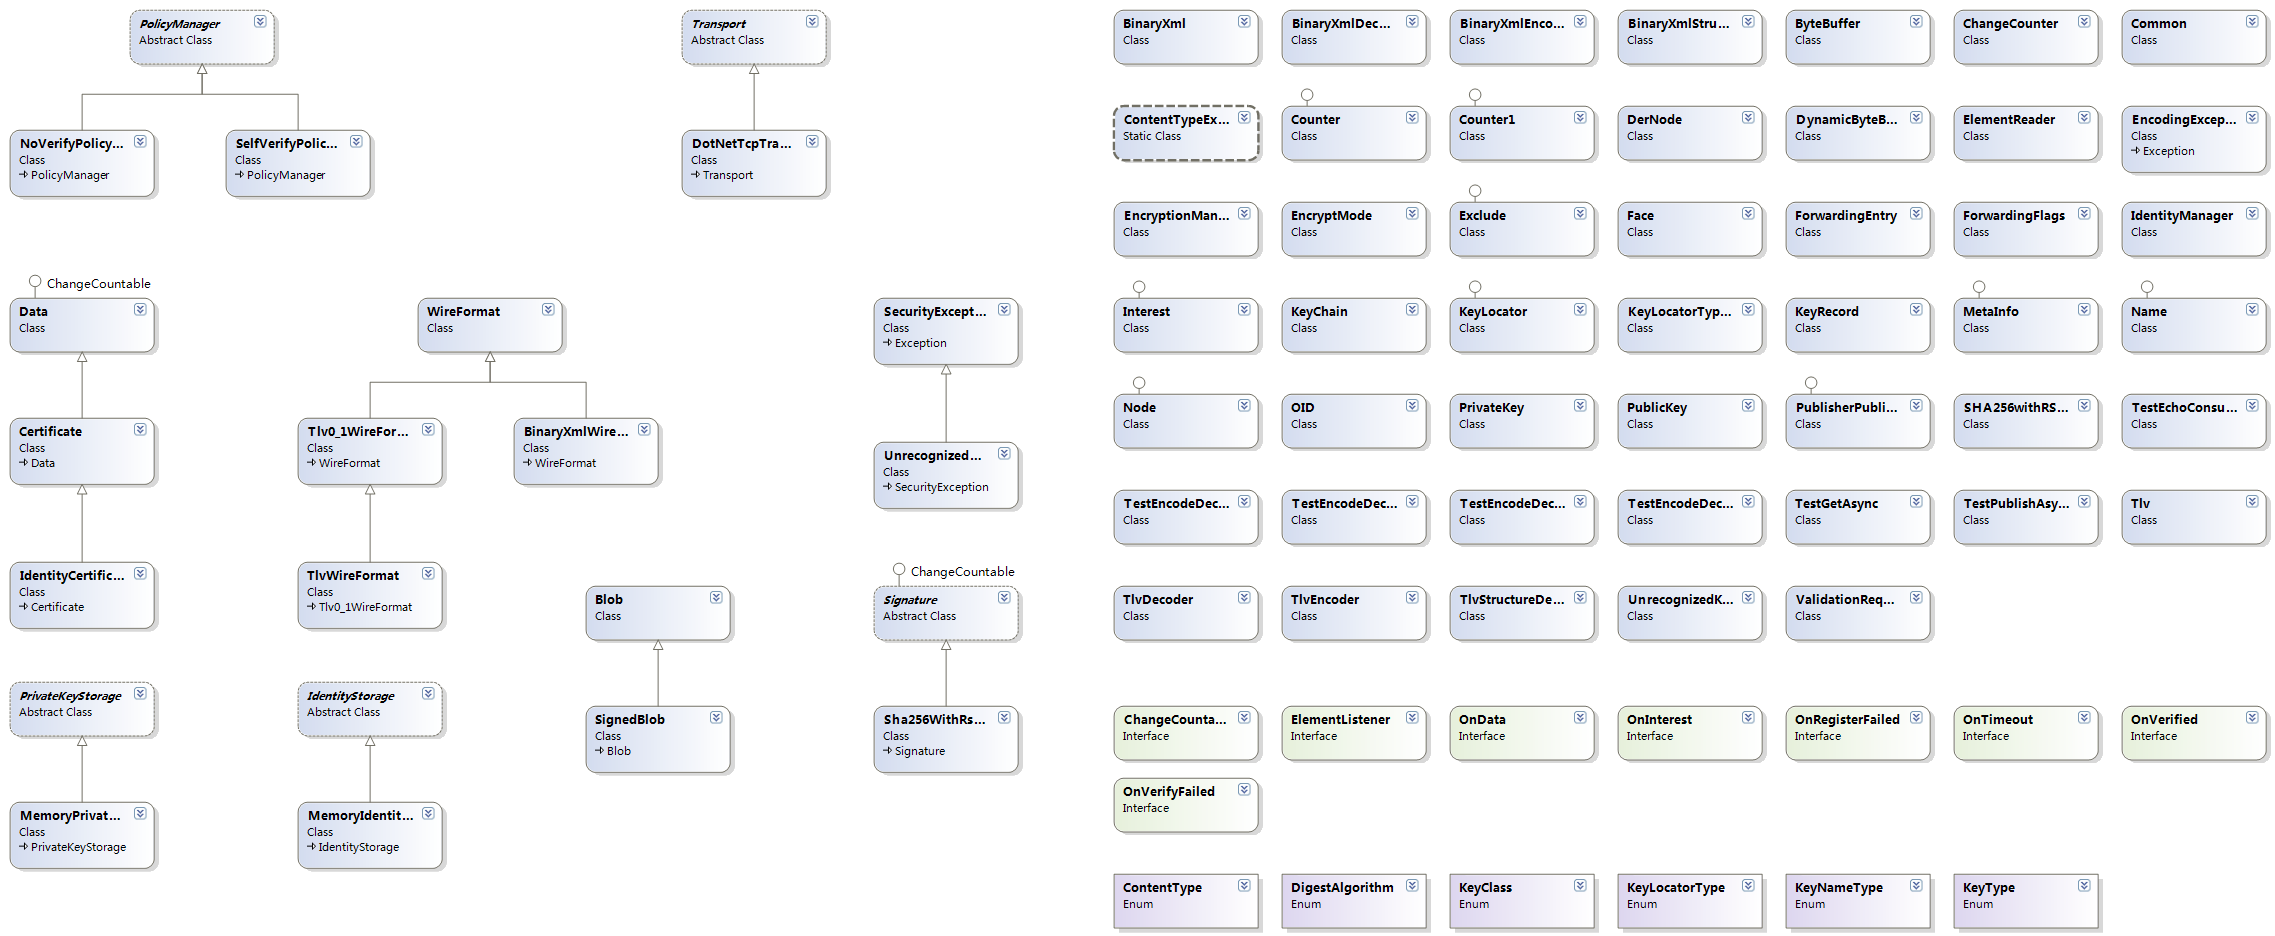
\includegraphics[width=0.95\textwidth]{TranslatedJndn.png}
	\caption{开发者函数库的类图描述}
	\label{fig:CCLClassDiagram}
\end{figure}
\par
由于篇幅限制,各个类的成员、方法和功能在此无法一一展开或描述,而简单应用开发中使用的重要的类在\ref{CCLSection}中已经有所介绍,在此不再赘述。

\section{设计详述}
\par
本部分详细叙述应用设计和工作流程。
\par
NDN应用设计的重要环节是命名空间(Namespace)的设计,为了达到局部性和可拓展性的目标,提供全局共享的命名空间是必要的。同时,由于NDN交互是通过数据请求和数据问答实现的,应用设计中应当考虑的问题是节点应该问网络怎样的问题,从而既在表达上没有二义性,又能尽量多的提供路由可用的信息,减少广播,提高效率。
\par
在游戏应用的同步用例中,对于每个节点,两个自然的问题是谁在我的附近,和它在哪里,在做什么。两个问题的结构对应着两个步骤,其优势在于, 问题一为问题二提供有助于路由的节点名称,从而经过网络节点模型的优化后,问题二的实际传输类似于单播。对于问题一,为了发现哪个对象在给定节点的附近,定期的广播数据请求是必要的。为了使命名空间可以共享,本文采取了对整个虚拟空间的静态八叉树划分。对于问题二,本文利用传统的NDN请求、应答交互实现位置、行动的更新。
\subsection{八叉树划分}
\par
虚拟环境的八叉树(Octree)\cite{OctreeRef}划分将整个三维虚拟环境划分为八个均等的立方体,对于每个立方体将其均等的划分为八个更小的立方体,以此类推,直到达到提前预设的层数。图\ref{fig:Octree}展示此划分。
\begin{figure}[h!]
	\centering
	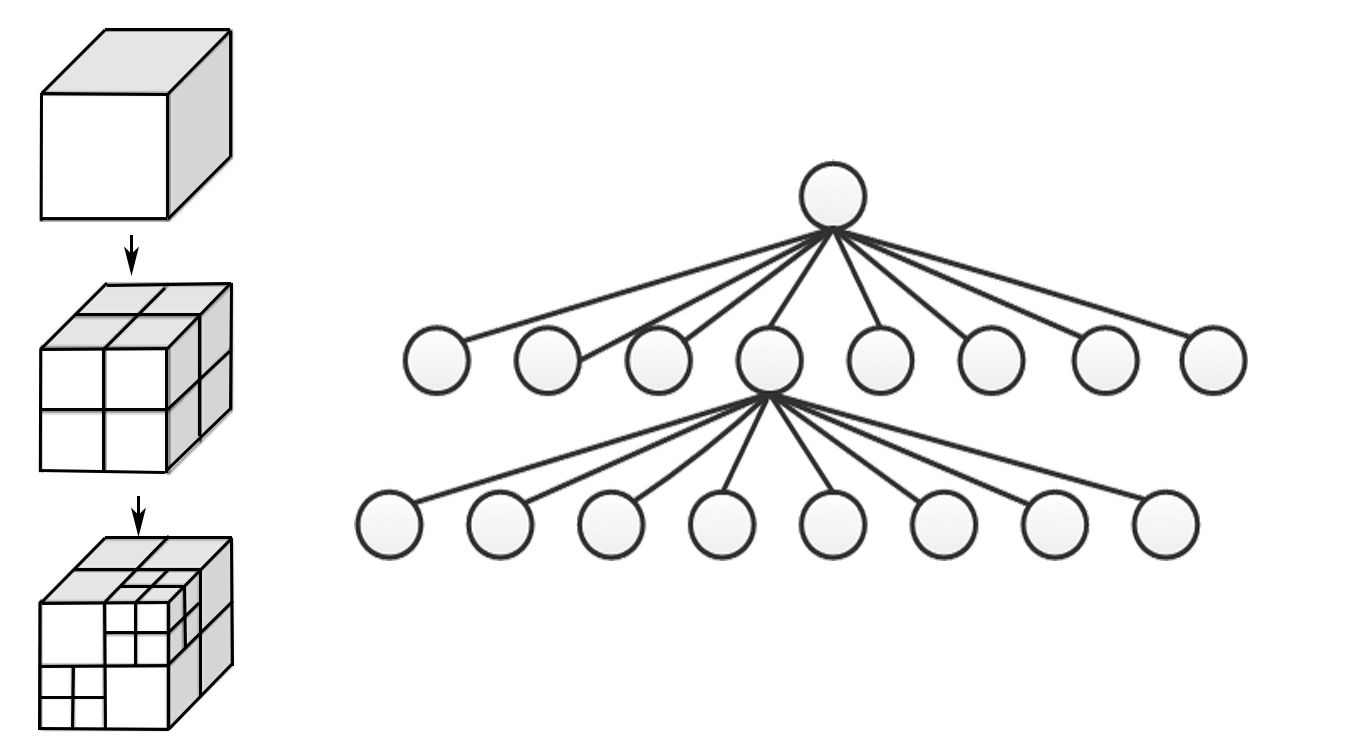
\includegraphics[width=0.75\textwidth]{Octrees.png}
	\caption{虚拟环境的八叉树划分}
	\label{fig:Octree}
\end{figure}
\par
如此划分得到的树是静态的和全局统一的。如果对于每一个立方体进行0~7的编号,整个虚拟环境中的每个大小立方体都可以用一组唯一的编号表示。通过将该序号编码在名称中,可以使名称表示特定的立方体。因此,对应名称的数据得到发布后,不论存储在哪个节点,该数据的含义是全局统一的。根据八叉树的划分结果,可以将每个节点的球形感知范围近似的用大小立方体表示。八叉树划分带来的主要优势是全局共享的命名空间:当节点A希望了解哪些对象在自己周围时,它可以分别根据A已知的存在于A的感知范围内立方体的立方体编号构成数据请求。如果没有统一的八叉树划分,A将使用自己位置和半径表达兴趣。如此,语义上讲,问题从谁在特定的区域中,变成了谁在给定(x, y, z)的R范围内。对于前者的问题,别的对同样区域感兴趣的节点可以共享该请求对应的应答;而对于后面的问题,由于短时间内另一个节点在完全相同的坐标发出完全相同的请求的概率很低,因此可以认为该问题的应答将只能对该请求者有效。况且,除了利用排除过滤的选择符(Exclusion filter),较难确保节点获取完整的问题答案。然而利用了排除过滤选择符后,往往会导致名称过长。综上,后者可以认为不是共享的命名空间,而八叉树划分提供了共享命名空间(Shared namespace),提高了数据共享的可能性。 
\subsection{发现模块}
\par
发现模块同样遵循局部性的设计要求。该要求可以诠释为,每个节点在任一时刻只希望了解自己的k-R最近邻居,该邻居由当前网络环境中唯一的节点名标识。相对于用固定的半径限制每个节点的感知范围,用kNN的优势在于其可以更好的利用网络资源。在节点所处的环境对象密集时,节点可以只获取最近的k个对象的位置,避免占用过大带宽。反之,在环境对象稀疏时,节点可以发现更远的对象。从游戏设计的角度来理解,可以视为是动态的调整感知范围的大小。
\par
发现模块利用八叉树划分的结果。每个节点了解自己所在的三维坐标,从而可以得到自己所在的立方体的编码,以及自己感知范围内包含的立方体的编码。对于处于自己感知范围内的立方体,节点通过名称注册接收和其相关的名称集合问题。同样由于前缀注册,对名称对应的立方体不了解或是不感兴趣的节点不会收到对应的数据请求。
\par
为了提高数据应答的利用率,同时确保收到的信息是完整的,本文在广播发现数据请求的名称最后添加了知识表达(Knowledge expression)字段。知识表达字段可以是对应立方体中本地了解的名称集的哈希。收到带有知识表达的数据请求的节点可以根据名称中包含的对象名称集的哈希值和本地已知的对象名称集的哈希值进行对比。仅当对于某一立方体,本地的对象名称集不同于收到的对象名称集时,收到数据请求的节点用自己集合内的对象名进行回答。
\par
综上所述,发现模块的命名空间可以用图\ref{fig:BroadcastNamespace}描述。
\begin{figure}[h!]
	\centering
	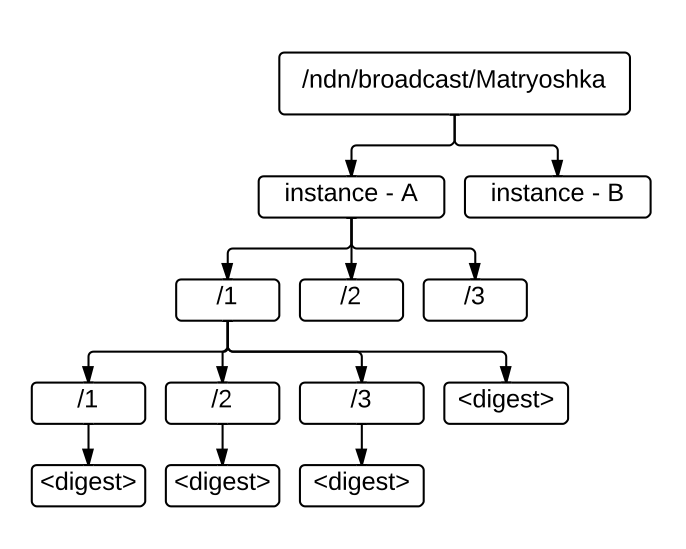
\includegraphics[width=0.70\textwidth]{DiscoveryNamespace.png}
	\caption{广播发现模块命名空间}
	\label{fig:BroadcastNamespace}
\end{figure}
\par
其中,最上层的时本应用的父命名空间;实体编号标识数据属于可能同时存在的多个实体中的哪一个(每一个对应一个独立的虚拟环境,不同实体中的游戏对象不需要发现对方);数字代表了八叉树立方体的编号;而digest代表了知识表达字段。
\par
收到的发现数据请求的数据应答应当由名称,所在的位置(最底层立方体)构成。由于没有任何一个节点是对名称中的立方体负责的,收到了名称并不代表本地对于该立方体的名称集合是不完整或是不正确的。在收到名称后,节点应当利用该名称构建对象位置的数据请求,从而真正确认是否本地的集合是不完整的。
\par
这样的哈希对应数据的表示方式体现了一个立方体的状态同步的步进过程,同时体现了将数据同步和状态同步分离的思想。相对于不把哈希值放在名称中的命名空间,这样的设计使得数据应答变得与数据存储位置无关。假设名称中没有哈希值,节点A在收到节点B关于立方体c的名称后,A没有办法确定B的答复是否准确。当A再次或是别的节点D同样表示对立方体c的请求后,如果请求经过了A、B间的缓存,获得的数据应答可能是B最初回复给A的不正确的,或是已经过时了的应答。
\par
然而上例体现了步进过程存在的一个问题。当一个节点的感知范围开始包括某一新的立方体时,该节点在获取到该立方体的最新信息前,可能会根据缓存中的内容给出的回复,对该立方体的历史状态进行遍历,直到获得最新状态。这样带来的问题是需要经过多个往返时间取得最新的状态。考虑到实时性的需求,本文利用ndnd-tlv支持的一项新选择符“必须为新鲜的“(Must be Fresh Child Selector)\footnote{参考在线文档,http://named-data.net/doc/ndn-tlv/interest.html}来减少获得过时信息的可能性。通过预设一个名称发现数据应答的新鲜时间,并且指定名称发现数据请求为”必须为新鲜的“,可以有效的通知缓存,本数据应答在多长时间内是有代表性的,在新鲜期过去后,该数据应答可以认为是过时的,不可以再次用来满足数据请求。
\par
根据上述逻辑,图\ref{fig:DesignSSD}展示了节点A通过节点B发现节点C的工作流程,在此给出作为发现模块的总结。
\begin{figure}[h!]
	\centering
	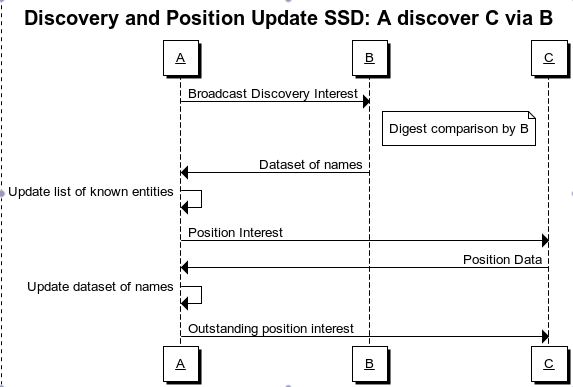
\includegraphics[width=0.70\textwidth]{SystemSSD.png}
	\caption{节点A通过B发现C的时序图}
	\label{fig:DesignSSD}
\end{figure}
\subsection{更新模块}
\par
每一个节点应当注册和自己的对象有关的数据请求前缀名称,即注册前缀包含自己的对象的名称的名称。
\par
发现模块将带来一系列的<对象名称-所在立方体编号>对。对于每一个名称,利用其构成位置数据请求(Position interest)和动作数据请求(Action interest),并向网络发送。利用之前所述的前缀注册过程,每一个的节点应当收到对自己位置的数据请求,对此该节点可以准确的作答。由于答案同样具有实时性的限制,在位置请求的数据应答中同样做以新鲜时间的设置,同时要求位置请求只获取新鲜的数据。
% Sample names
\par
综上所述,更新模块的命名空间如图\ref{fig:PositionUpdateNamespace}所示。
\begin{figure}[h!]
	\centering
	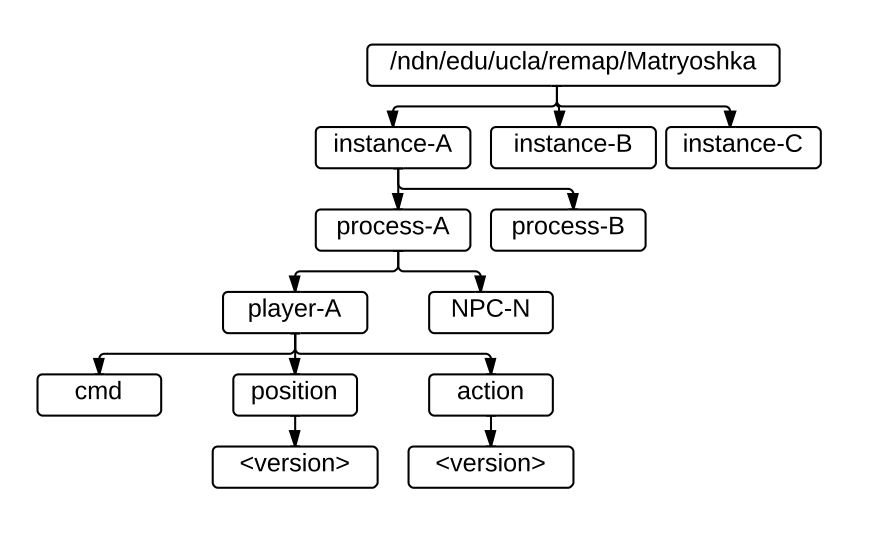
\includegraphics[width=0.90\textwidth]{PositionNamespace.png}
	\caption{更新模块命名空间}
	\label{fig:PositionUpdateNamespace}
\end{figure}
\par
为了确定是否需要对本地的立方体-名称集合表进行更新,更新模块应当记录每一个对象之前是否有被发现,以及其上一次被发现的位置在哪里。由于发现模块并不决定一个对象是否在其所述的立方体中,更新模块将根据几类不同的数据应答做出决定。
\par
收到了位置,位置属于自己感兴趣的立方体,位置所在的立方体和上次位置所在的立方体一致:应答节点在自己的兴趣范围内运动,本地应当渲染其现所在位置,并利用其现所在位置更新其上次位置。
\par
收到了位置,位置属于自己感兴趣的立方体,位置所在的立方体和上次位置所在的立方体不一致:应答节点从自己感兴趣的一个立方体进入了感兴趣的另一个立方体,本地应当渲染其现所在位置,并利用其现所在位置更新其上次位置,同时将其从之前的立方体的名称集合中移除,将其加入之后的立方体的名称集合。
\par
收到了位置,位置属于自己感兴趣的立方体,没有上次记录:新发现并确定应答节点存在,本地应当渲染其现所在位置,并利用其现所在位置设置其上次位置。
\par
收到了位置,位置不属于自己感兴趣的立方体,位置所在的立方体和上次位置所在的立方体不一致:应答节点离开了自己的感知范围,应当将其从上次的立方体的名称集合中删除,并不再渲染。同时把该节点从需要进行位置请求的节点名称列表中移除。
\par
收到了位置,位置不属于自己感兴趣的立方体,没有上次记录:收到了无关应答,可能由仍然处于预设的新鲜期内,但是实际已经过时的发现请求的应答导致。此情况下应该把该节点从需要进行位置请求的节点名称列表中移除。
\par
没收到位置,有上次记录:节点可能掉线,或是短时间无法应答。再次发出同样的数据请求。如果没有收到数据应答的次数达到预定阈值,则认为节点掉线,不再渲染,将其从上次位置对应的立方体的名称集合中删除。同时,把该节点从需要进行位置请求的节点名称列表中移除。
\par
没收到位置,没有上次记录:可能收到了错误、过时的节点名称,或是待被发现的节点暂时无法应答 。再次发出同样的数据请求。如果没有收到数据应答的次数达到预定阈值,则认为该节点不存在,把该节点从需要进行位置请求的节点名称列表中移除。
\section{面向对象设计}
\setcounter{subsubsection}{0}
\par
在完成了对交互过程和工作流程的描述后,本文从实现的角度描述设计方案具体包含的组件。本文采取的实现是面向对象的,图\ref{fig:DIscoveryModuleClassDiagram}为发现、更新模块项目实现的类图,由于篇幅限制没有展开。
\begin{figure}[h!]
	\centering
	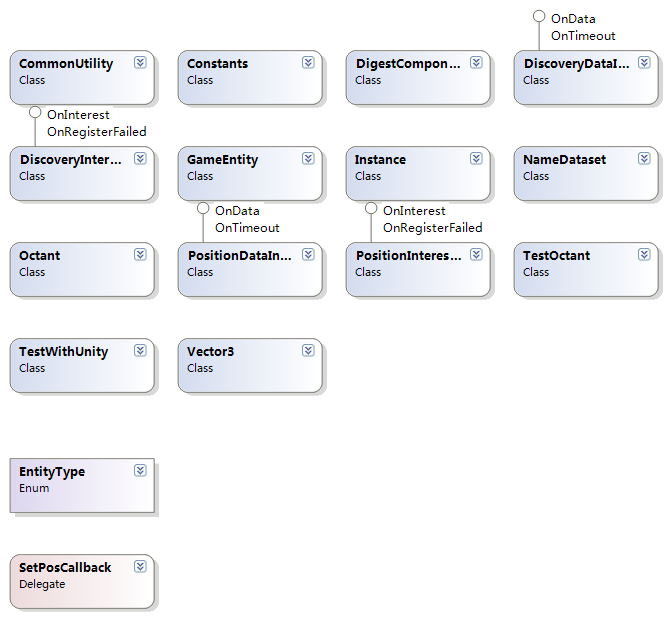
\includegraphics[width=0.70\textwidth]{DiscoveryModule.png}
	\caption{同步模块的类图描述}
	\label{fig:DIscoveryModuleClassDiagram}
\end{figure}
\par
其中主要类的功能介绍如下。
\subsubsection{实体类(Instance)}
包含了请求、应答接口;存储本地的八叉树结构和每个树节点对应的哈希值和名称集;存储本地对象的相关信息和已知的对象列表;决定向哪个立方体和哪个对象发出数据请求;并在开始/结束时创建/终止线程实际进行发现/更新。
\subsubsection{发现请求接口类(DiscoveryInterestInterface)}
负责发现请求相关的请求处理。继承自OnInterest和OnRegisterFailed,重载请求处理函数。根据传入的Instance的引用对Instance中的本地八叉树结构中对应立方体的名称集和其哈希值进行访问并对收到请求做以应答。
\subsubsection{发现应答接口类(DiscoveryDataInterface)}
负责发现请求相关的应答处理。继承自OnData和OnTimeout,重载应答处理函数。根据传入的Instance的引用对Instance中的需要发出请求的对象列表进行书写。这里涉及到需要发出请求的对象列表的跨线程写入,因此需要互斥锁。
\subsubsection{更新请求接口类(PositionInterestInterface)}
负责位置请求相关的请求处理。继承自OnInterest和OnRegisterFailed,重载请求处理函数。根据传入的Instance的引用对Instance中的本地对象进行访问并对收到请求做以应答。
\subsubsection{更新应答接口类(PositionDataface)}
负责位置请求相关的应答处理。继承自OnData和OnTimeout,重载应答处理函数。根据传入的Instance的引用对Instance中的渲染对象列表进行书写。这里涉及到渲染对象列表的跨线程写入,因此需要互斥锁。
\subsubsection{八叉树节点类(Octree)}
负责八叉树节点及其名称集和哈希值的存储。本文中的树以左子右兄的结构存储。Instance中包含了此类型的八叉树根节点。
\subsubsection{游戏对象类(GameEntity)}
游戏对象类封装了游戏对象相关的属性,例如其名称、类型和位置,以及对游戏渲染函数等函数的回调入口。该类应当抽象出一个对象类,从而降低和游戏应用的耦合度。
\section{本章小结}
本章详细描述了命名空间,系统的设计逻辑。设计方案首先对虚拟环境进行统一的八叉树划分,形成共享命名空间,然后对划分得到的每个立方体进行同步。同步的过程为节点定时广播利用该立方体编号组成的名称以及名称集状态构成的发现数据请求。收到请求的节点返回名称集。发出请求的节点根据返回的名称组成含路由信息的位置请求,并利用该位置请求最终确定是否进行渲染,以及是否保持位置、动作的同步或作出怎样的更新。
